\chapter{Architettura e sviluppo del sistema}
Come esposto nei capitoli precedenti, le reti IoT nascono con l'intenzione di mettere in comunicazione potenzialmente milioni di sensori e dispositivi. Questi dispositivi possono avere interfacce differenti, avere hardware differente e possono assolvere a compiti completamente differenti l'uno dall'altro. L'obiettivo è quello di sviluppare un sistema centralizzato in grado di monitorare questi smart objects, su richiesta dell'utente, e pubblicare cambiamenti di stato o valori periodici su canali familiari all'utente, che può consultare con semplicità.
\\Il sistema deve necessariamente essere strutturato considerando le seguenti parole chiave:
\begin{itemize}
\item \emph{Scalabilità}: data la potenziale mole di nodi da osservare è mandatorio che il sistemi scali correttamente.
\item \emph{Portabilità}: il sistema deve essere slegato da vincoli hardware e soprattutto software relativi ai sistemi operativi, data la molteplicità di realtà presenti oggi sul mercato, potendo potenzialmente essere portato in sistemi cloud più estesi.
\item \emph{Interoperabilità}: il sistema deve necessariamente essere interoperabile, ovvero deve poter operare con il maggior numero possibile di nodi e dispositivi, cercando di astrarre il più possibile dal tipo di dati trattati e dalle sue caratteristiche intrinseche. Il sistema deve inoltre essere in grado, potenzialmente, di poter restituire i dati su differenti canali ed essere sempre pronto all'espansione e alle modifiche in tal senso.
\end{itemize}
Il sistema sarà quindi composto da tre unità fondamentali:
\begin{itemize}
\item La cloud Java
\item Il DBMS
\item L'interfaccia Web
\end{itemize}
Tutte le componenti sono state pensate e sviluppate per poter essere indipendenti e intercambiabili, nei limiti del possibile, per ottenere un sistema flessibile e facilmente manutenibile.
\vspace{1.0cm}
\begin{figure}[h]
\centering
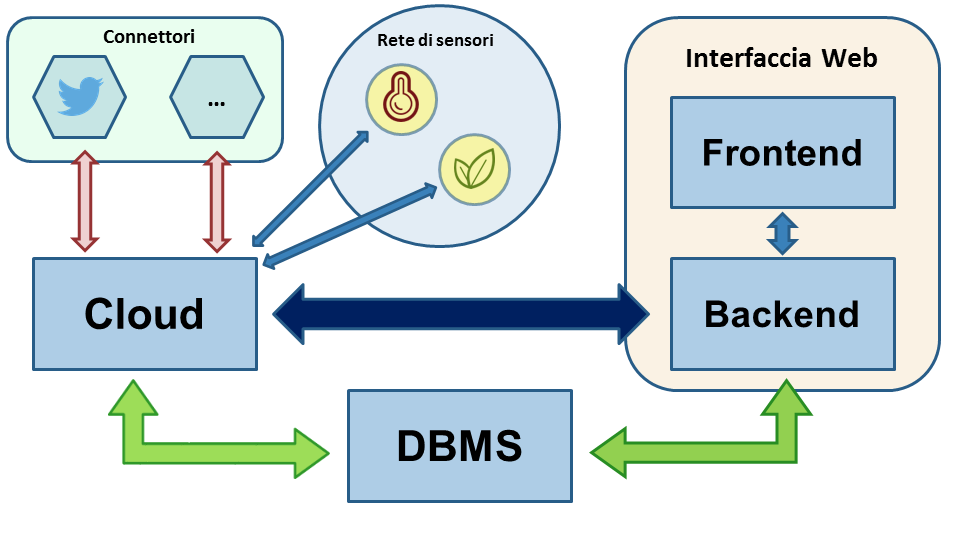
\includegraphics[width=\textwidth]{immagini/cloud.png}
\caption{\textit{L'architettura del sistema di monitoraggio}}
\end{figure}

\section{La cloud Java}
La cloud Java è certamente la componente più importante dell'intero sistema: essa si occupa infatti di effettuare il monitoraggio delle risorse tramite protocollo CoAP su richiesta dell'interfaccia Web, e di pubblicare, periodicamente o al succedersi di un evento, i dati ottenuti su canali definiti dall'utente, chiamati \textit{connettori}.
\\Le richieste dall'interfaccia Web verso la cloud sono fatte mediante chiamate remote, utilizzando XML-RPC.
\\È stato scelto il linguaggio Java principalmente per la sua caratteristica intrinseca di portabilità: è infatti sufficiente avere la JVM (Java Virtual Machine) per far girare la cloud, non essendoci chiamate particolari al sistema operativo e non effettuando alcuna operazione dedicata su hardware specifico. Il linguaggio Java inoltre, grazie al livello di astrazione eccezionale che fornisce, ha permesso uno sviluppo veloce e abbastanza ordinato, anche grazie all'ampia disponibilità di librerie, sia integrate che facilmente reperibili da terze parti. 
\\La cloud è sostanzialmente composta da un server XML-RPC, la classe {\tt Server}, che è sempre in esecuzione e disponibile, che riceve le chiamate remote dall'interfaccia; a questo punto le chiamate vengono passate all'handler XML-RPC, la classe {\tt CoapHandler}, che a sua volta le smista al {\tt CoapAgent}, un thread particolare di cui esiste una sola istanza, che è un po' l'esecutore materiale della richiesta: si occupa infatti di creare l'azione richiesta nel database, configurare il connettore e lanciare il thread specifico che si occuperà di monitorare la risorsa indicata dall'utente. L'{\tt Agent} ha anche il compito di interrompere l'esecuzione di questi thread di monitoraggio se richiesto e, anche se in piccola parte, si occupa di controllare che ogni thread non sia "pendente", ovvero che non sia rimasto in esecuzione nonostante la sua azione non sia più presente nel database.
\begin{figure}[pt]
\centering
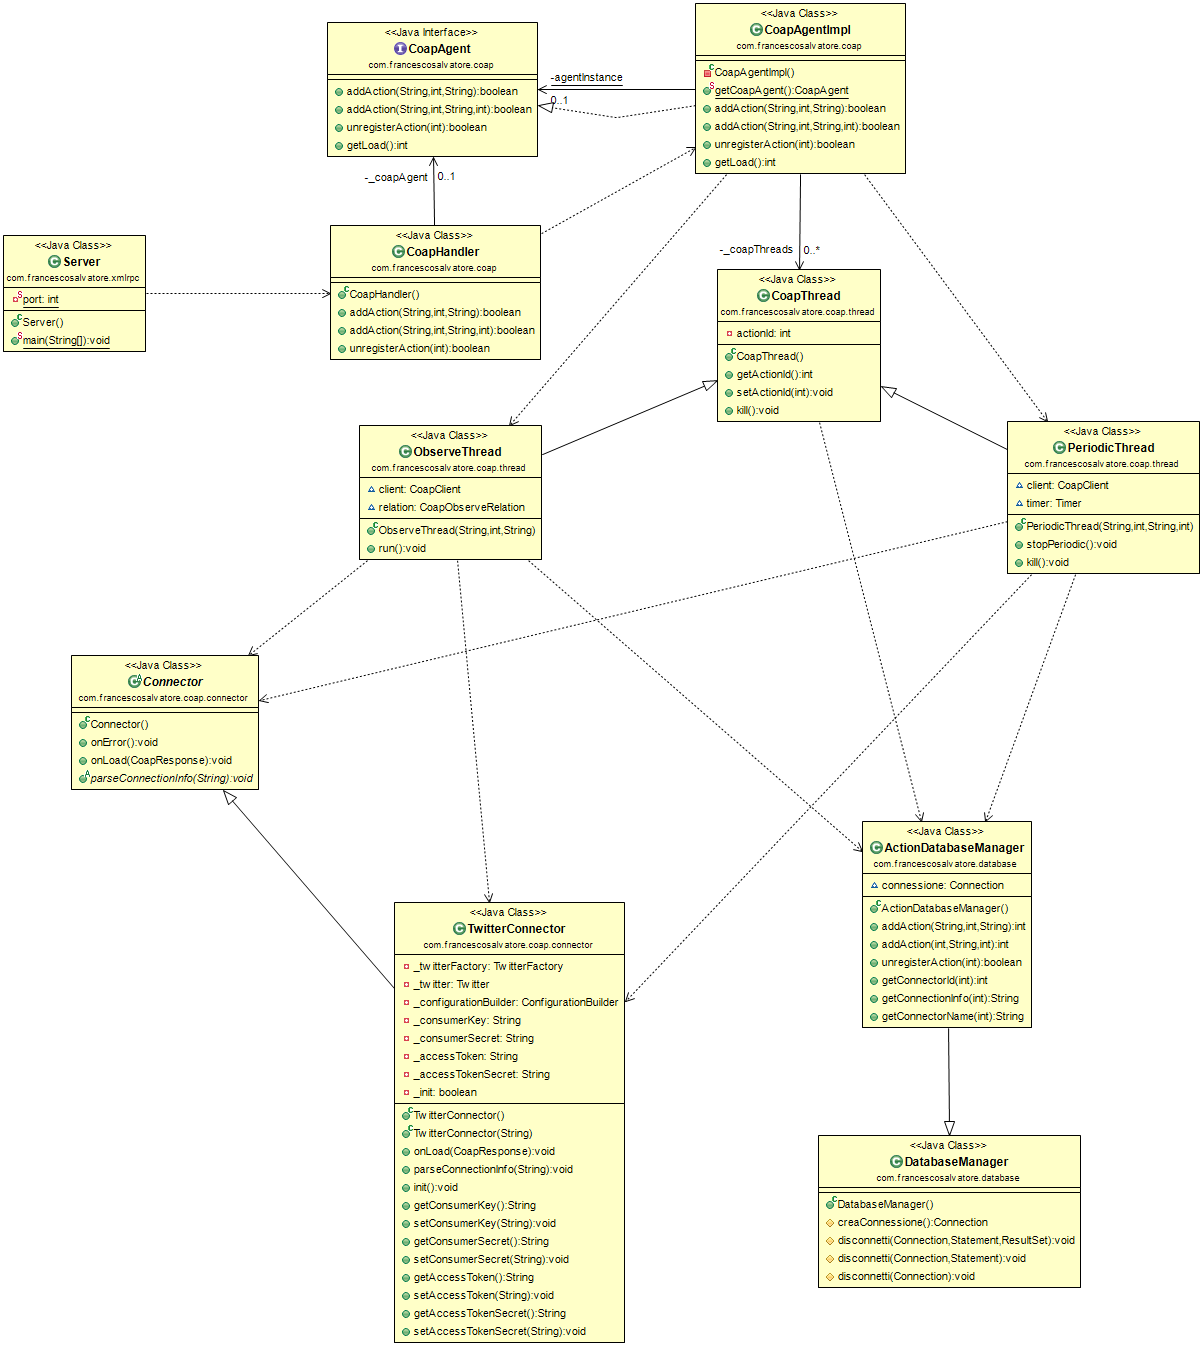
\includegraphics[width=\textwidth]{immagini/uml.png}
\caption{\textit{Il diagramma UML delle classi della cloud Java}}
\end{figure}
\\\\Possiamo trovare due tipi, per il momento, di thread di monitoraggio:
\begin{itemize}
\item {\tt ObserveThread}: si mettono in ascolto su di una risorsa e, in caso di cambiamento di evento sulla risorsa, lo notificano al connettore scelto.
\item {\tt PeriodicThread}: controllano periodicamente il valore della risorsa indicata, secondo il tempo richiesto dall'utente, e notificano il valore al connettore scelto.
\end{itemize}
I connettori quindi ricevono il valore e lo elaborano, a seconda del comportamento del connettore stesso.
\\\\Il DBMS scelto è MySQL, per alcune semplici ragioni: è gratuito, nella sua versione base, è semplice da installare ed è multipiattaforma, oltre che essere conforme agli standard ANSI SQL e ODBC SQL. Per la connessione e la gestione è stato però scelto di utilizzare il driver \textit{JDBC} (Java DataBase Connectivity), che permette di creare un livello di astrazione tra le chiamate al database e il database stesso, garantendo la possibilità di poter cambiare DBMS con semplicità e in maniera "indolore", senza quindi dover radicalmente modificare la struttura o il codice stesso del programma. Questo accorgimento ci permette di poter spaziare tra i DBMS che supportano ODBC e per i quali esiste il driver specifico, tra i quali troviamo i maggiormente utilizzati PostgreSQL, Oracle, Microsoft SQL Server, Sybase, DB2, SQLite e molti altri.
\\Vi è inoltre una classe che si occupa di implementare l'astrazione dal database, che è la classe {\tt DatabaseManager}.
\\\\Per la comunicazione verso le risorse, ovvero gli smart objects, è stato scelto il protocollo CoAP. CoAP è semplice, garantisce un basso overhead ed è in grado di funzionare adeguatamente sia su reti IPv4 che IPv6, garantendo una buona interoperabilità del nostro sistema e delle reti monitorate con infrastrutture e architettura già presenti. CoAP inoltre presenta la possibilità di "osservare" una risorsa, tenendo costantemente monitorato il suo valore ed essendo avvisati dalla risorsa stessa in caso di cambiamento, evitando alla cloud di dover effettuare un polling costante sulla risorsa stessa, che sarebbe eccessivamente gravoso sia in termini di risorse di calcolo sia in termini di traffico di rete generato (ricordiamo che spesso questi smart objects sono all'interno di reti a ristretta larghezza di banda ed effettuare polling costanti anche su pochi dispositivi significherebbe saturare queste reti).
\\La libreria che ci permette di effettuare queste operazioni su CoAP è Californium, un framework completo che permette di lavorare sia in modalità client che server, sviluppato da Matthias Kovatsch. Californium è passata con successo all'ETSI (European Telecommunications Standards Institute) IoT PlugTest, un test di interoperabilità tra sistemi di smart objects. Californium è potente ma allo stesso tempo leggero e facilmente gestibile. Inoltre permette di simulare smart objects su differenti reti, funzionalità che ho ampiamente utilizzato per emulare una rete di sensori.

\subsection{XML-RPC}
Considerando gli obiettivi del sistema di portabilità e interoperabilità era necessario pensare ad una modalità standard per poter mettere in comunicazione l'interfaccia Web e la cloud. È stata fatta quindi la scelta di utilizzare un sistema stile web-service, che garantisce di poter sostituire l'interfaccia Web o la cloud utilizzata con un qualunque sistema in grado di effettuare e ricevere chiamate remote. In particolare la scelta è caduta su XML-RPC, protocollo che utilizza il linguaggio XML per incapsulare le chiamate e HTTP come modalità di trasporto, per ragioni di semplicità: XML-RPC è infatti più semplice e leggero di altri sistemi RPC come SOAP, non necessita di definire encoding particolari e non necessita di creare le descrizioni del servizio WSDL (Web Service Description Language), superflue agli scopi di questo sistema.
\\Il funzionamento di XML-RCP è abbastanza elementare: le chiamate di funzione, con relativi argomenti, vengono serializzate in linguaggio XML, che viene poi passato al server tramite protocollo HTTP, che li deserializza. Questo meccanismo rende veramente agevole il processo di chiamata remote ed è estremamente compatibile con le tecnologie esistenti, in quanto sia XML che HTTP sono ampiamente supportati.
\\Esistono in fatti decine di implementazioni di questo protocollo ed è stato scelto di utilizzare la libreria \textit{Apache XML-RPC2} per quanto riguarda la cloud Java, mentre per l'interfaccia Web è stato scelto di utilizzare il modulo integrato in PHP (dalla versione 5.0 in su).

\subsection{I connettori}
Uno dei problemi dell'utilizzare reti di sensori estese è sicuramente quello di ottenere i dati in maniera semplice, chiara, leggibile anche da un utente consumatore senza particolare esperienza nel campo tecnologico, e certamente una delle funzionalità più interessanti è quella di essere avvisati dalla rete di sensori quando sussiste un determinato evento (un cambiamento di un valore di temperatura, oppure un movimento rilevato da un sensore di movimento ecc...). È quindi utile poter utilizzare canali comodi e familiari all'utente, come per esempio i social media, per pubblicare i dati e da qui l'idea di sviluppare il sistema modulare, pronto per impiantare sopra di esso dei \textit{connettori}, ossia delle interfacce di astrazione che si occupano di ricevere il dato grezzo ed elaborarlo, secondo la propria specifica: il connettore di Twitter, per esempio, potrebbe pubblicare un tweet, o quello di Facebook un messaggio sulla propria bacheca; o ancora un connettore per Telegram, la nota app di messaggistica, potrebbe inviarci un messaggio sul nostro smartphone oppure il connettore mail potrebbe inviare una email al nostro indirizzo personale e via dicendo.
\\La cloud Java offre quindi una interfaccia {\tt Connector} che definisce alcuni metodi e proprietà che ogni connettore deve avere, ma lascia ampia libertà implementativa, permettendo una customizzazione abbastanza elevata del comportamento del singolo connettore.
\\Nel sistema cloud in questione è stato implementato un solo connettore, quello di Twitter, che è in grado di pubblicare sulla propria timeline un tweet contenente il dato estratto dalla risorsa monitorata.

\subsection{Le REST APIs e la libreria Twitter4J}
Twitter mette a disposizione degli sviluppatori una interessante API (Application Programming Interface) REST, ovvero una interfaccia HTTP che utilizza il modello URL per ricevere le richieste dall'applicazione e restituisce i risultati in formato JSON. Le Twitter APIs utilizzano un sistema di autenticazione denominato OAuth, ed in particolare la versione 2.0, un protocollo che permette di ottenere un discreto livello di sicurezza per ottenere dati particolari. Il protocollo OAuth è standardizzato ed è stato recepito da IETF nel RFC 6749.
\\Le REST APIs permettono, seppur con qualche limitazione, di effettuare operazioni sui dati Twitter ma necessitano di chiavi di autenticazione che solo l'utente stesso può fornire. In questo modo si garantisce che nessuna applicazione di terze parti possa, senza l'autorizzazione del proprietario dell'account, effettuare pubblicazioni a suo nome.
\\Per l'interfacciamento con le REST APIs è stato scelto di utilizzare la libreria \textit{Twitter4J}, sviluppata da Yusuke Yamamoto e distribuita sotto Apache License 2.0. La libreria permette di effettuare, direttamente da Java, chiamate alla API, supporta nativamente OAuth ed è semplice da integrare, non richiedendo alcuna dipendenza aggiuntiva.

\section{L'interfaccia Web}
Come è importante per l'utente poter accedere ai dati della rete di smart objects tramite canali a lui familiari, è altrettanto importante fornirgli una modalità di configurazione semplice ed intuitiva, che sia fruibile tramite il maggior numero possibile di dispositivi nei modi più chiari possibile.
\\È naturale quindi che sia stato scelto l'ambiente Web per lo sviluppo dell'interfaccia, in quanto altamente raggiungibile sia da dispositivi classici, come PC, sia da dispositivi mobili, come smartphone e tablet, sia da altre tipologie di dispositivi che sempre più sono equipaggiati con interfacce di rete e applicazioni browser, come smart TV, Set-top-box, console videoludiche ecc...
\\L'idea è quella, anche qui, di sviluppare un sistema di backend che sia altamente compatibile con il maggior numero possibile di architetture e sistemi, che sia scalabile e facilmente manutenibile.
\\Sebbene inizialmente sia stato preso in considerazione di sviluppare l'interfaccia Web al di sopra della cloud, sfruttando tecnologie offerte dall'ambiente Java come Tomcat e le Servlet, ci si è reso conto che questo avrebbe compromesso eccessivamente la modularità dell'intero sistema, legando troppo fortemente la componente server all'interfaccia. PHP è sembrata quindi la scelta più logica: è semplice, relativamente leggero, altamente compatibile ed è supportato da tutti i maggiori web-server in circolazione, oltre che essere una tecnologia leader in campo Web.
\\PHP (acronimo anagrammato di Hypertext PreProcessor) è un linguaggio stile C nato a metà degli anni '90 per semplificare la costruzione di applicazioni Web che non necessitassero di avere esigenze particolari. Nel tempo ha subito grandi trasformazioni ed oggi è un linguaggio assolutamente completo e molto potente. PHP è un linguaggio interpretato, almeno nella sua implementazione standard, lo Zend Engine, ma ha al suo interno complessi sistemi di caching che ne aumentano notevolmente le perfomance.
\\\\Troviamo quindi anche qui, come per la cloud, un orientamento agli oggetti, dove le classi {\tt DatabaseManager} e {\tt LoginManager} gestiscono rispettivamente l'accesso al database e le operazioni di validazione del login.
\\Come per la parte cloud anche qui si è scelto un approccio aperto verso la gestione del DBMS, utilizzando i driver PDO offerti dal pacchetto PHP: PDO (PHP Data Objects) è un'interfaccia simile ad ODBC (da cui eredita anche alcune componenti), pensata per astrarre le operazioni sul database dal DBMS. Le operazioni sono quindi preparate in linguaggio SQL standard (compatibile con la maggior parte dei database SQL) e passate al PDO driver corretto, nel nostro caso MySQL. PDO è integrato a partire da PHP 5.1.
\\\\Attraverso l'interfaccia Web, dopo aver effettuato il login, necessario al fine di autenticare l'utente, è possibile configurare i connettori (per il momento è disponibile solamente Twitter), immettendo le proprie credenziali che saranno necessarie al connettore per effettuare le operazioni specifiche. Una volta configurati, tramite apposita form, si può registrare una \textit{azione}: l'azione può essere di tipo \textit{observe} o \textit{periodic}, a seconda che si voglia effettuare un monitoraggio costante della risorsa oppure periodico, ed è possibile inserire la URL della risorsa da osservare, oltre che impostare altri parametri utili. Una volta premuto il pulsante di aggiunta dell'azione, i dati inseriti vengono serializzati e viene effettuata una chiamata RPC al metodo {\tt addAction} della classe {\tt CoapAgent} sulla cloud.
\\Nella dashboard principale troviamo invece l'elenco delle azioni registrati, con la possibilità di eliminarle, e una sidebar che contiene tutti i messaggi pubblicati dai vari connettori in tempo reale.

\subsection{La libreria TwitterOAuth}
L'interfaccia Web è anche munita di una sidebar, nel suo frontend, da cui è possibile visionare i dati pubblicati sui vari connettori. Per il connettore Twitter è stata utilizzata la libreria TwitterOAuth sviluppata da Abraham Williams per interfacciare in maniera semplice e robusta le Twitter REST APIs. La libreria prevede un flusso di autenticazione sicuro ed è stata sviluppata secondo il paradigma della programmazione ad oggetti, che la rende ordinata e semplice da utilizzare.
\\Questa libreria è stata preferita ad altre principalmente per la sua semplicità, la sua incredibile capacità di customizzazione e la sua piena compatibilità con le recenti APIs 1.1, da poco rilasciate, ed è inoltre compatibile e testata per funzionare anche su PHP 7, anche questo di recente rilascio.
\\TwitterOAuth è inoltre in grado di effettuare automaticamente il parsing dei risultati JSON, restituendo oggetti PHP più facilmente gestibili.

\subsection{Il framework Bootstrap}
Come già sottolineato uno degli aspetti importanti dello sviluppo di questo sistema di monitoraggio è certamente l'usabilità e non era quindi possibile disegnare un'interfaccia utente che non fosse in linea con le più moderne tecnologie e compatibile con il maggior numero possibile di dispositivi. Si è scelto quindi di utilizzare il framework Bootstrap per lo sviluppo dell'interfaccia grafica. Bootstrap è un framework di sviluppo Web per frontend, sviluppato da Mark Otto e Jacob Thornton di Twitter e reso pubblico e open-source nel 2012. Giunto alla sua versione 4, permette di accellerare lo sviluppo di interfacce web tramite strumenti che semplificano le azioni di compatibilizzazione cross-browser e che automatizzano il responsive design, ovvero la capacità di una interfaccia web di adattare il proprio layout in base al tipo di dispositivo con cui si accede all'interfaccia stessa.
\\Il responsive design è una componente importante dell'accessibilità: sempre più spesso infatti i contenuti web vengono fruiti da dispositivi differenti l'uno dall'altro, talvolta con dimensioni dello schermo che potrebbero rendere la visualizzazione quasi impossibile se il layout fosse mantenuto uguale. Bootstrap si occupa quindi di ridimensionare, spostare e accorpare i componenti dell'interfaccia (bottoni, menù, contenitori ecc...) in base alle dimensioni dello schermo dell'utente, permettendo di mostrare un layout più chiaro e pulito e quindi facilmente utilizzabile.
